\chapter{Framework Valutati}
	Il primo passo necessario nella valutazione di questi framework è stato 
	chiarire bene il fine del loro impiego. Durante la fase di ricerca abbiamo 
	notato una gran confusione nell'attribuire a ciascun framework il tipo di
	applicazione che permetteva di realizzare. Spesso il fatto che 
	l'applicazione venisse eseguita all'interno di una componente nativa veniva 
	pubblicizzato come se il framework fosse in grado di creare una completa 
	applicazione nativa (anziché ibrida); in altri casi 
	veniva confuso il concetto di \crosscomp 
	(\hyperref[sec:nativapp]{vedi~\ref{sec:nativapp}}) con quello di 
	applicazione ibrida; in altri ancora non veniva mostrata la separazione 
	concettuale che vi è tra framework utili per la sola costruzione della 
	logica e dell'interfaccia grafica dell'applicazione e framework che 
	permettono d'incapsulare il contenuto web in una componente nativa creando 
	così un'applicazione ibrida.
	
	Allo scopo di dare ordine per descrivere al meglio le differenze tra i vari 
	framework abbiamo ritenuto opportuno suddividerli a seconda del tipo di 
	applicazioni che sono in grado di produrre.
	
	Abbiamo così classificato Titanium Appcelerator come framework per la 
	realizzazione di applicazioni native; Phonegap/Cordova, Rho Mobile e Sencha 
	Touch come quelli dediti alla creazione di applicazioni ibride; jQuery 
	Mobile, KendoUI Mobile e PhoneJS utili per implementare complete 
	applicazioni web e per la logica e l'interfaccia grafica di applicazioni 
	ibride.

	\section{Framework per Applicazioni Native}
		
		\subsection{Titanium Appcelerator}
		\label{sec:titanium}
			Titanium è una piattaforma gratis e open source di sviluppo di 
			applicazioni mobili che permette la creazione di applicazioni native
			\crossplat{} per iOS, Android, BlackBerry e Tizen usando il 
			linguaggio JavaScript. Usando JavaScript e HTML è anche possibile
			creare semplici applicazioni Web.
			
			Titanium agisce come un ponte tra i sistemi operativi nativi e il 
			codice dell'applicazione. La figura \ref{fig:ti_stack} illustra 
			questa architettura.
			\begin{figure}[h]
				\centering
				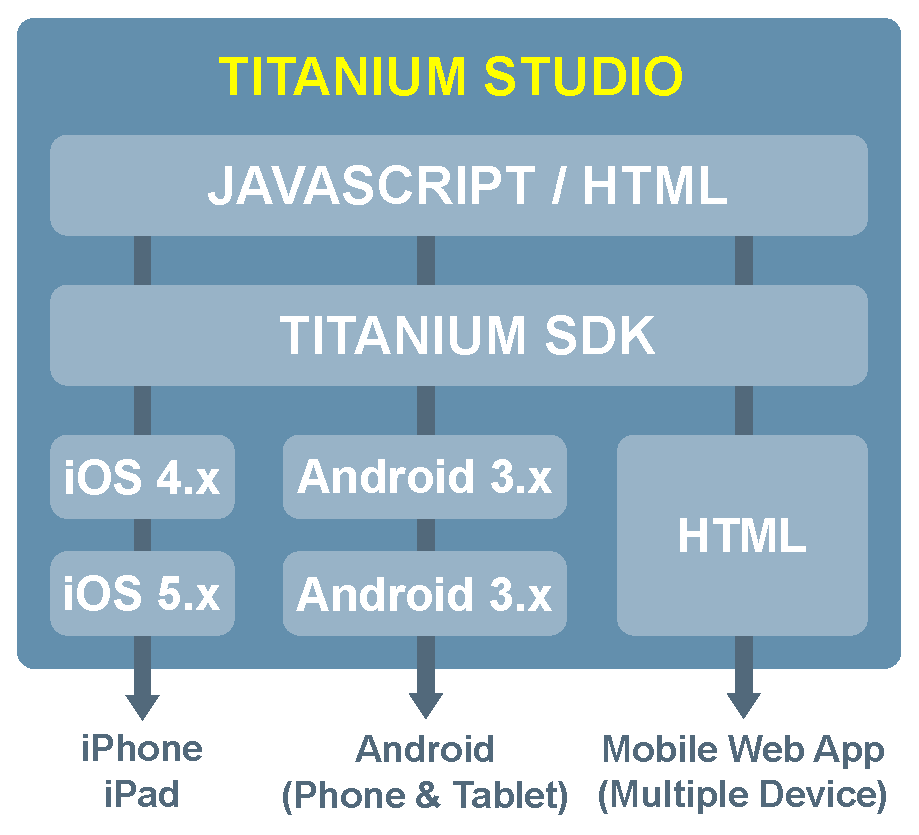
\includegraphics[keepaspectratio=true, width=12cm]{titanium-stack.eps}
				\caption{
					Architettura nello sviluppo di un applicazione \crossplat{} 
					mediante Titanium Studio.
				}
				\label{fig:ti_stack}
			\end{figure}
			In fondo alla pila si trova il sistema 
			operativo di destinazione: Android, iOS o il browser (per quanto 
			riguarda le applicazioni web); sulla cima troviamo il codice 
			dell'applicazione scritta in JavaScript e in mezzo trova posto
			Titanium SDK insieme alle proprie APIs. Utilizzando tali interfacce 
			nella propria applicazione è possibile fare azioni come mostrare la 
			fotocamera,	aprire nuove finestre, disegnare pulsanti, ecc. 
			
			Titanium è descritto come un framework \crosscomp{}\citep{Web:peptechlearn.blogspot.it} anche se l'uso che si fa di 
			questo appellativo in questo caso non è del tutto corretto. Come 
			spiega lo stesso amministratore delegato di Appcelerator Inc., Jeff 
			Haynie, in un intervento online su 
			\mbox{stackoverflow.com}\footnote{In quell'occasione era stato 
			chiesto proprio come Titanium potesse funzionare riguardo alla 
			creazione del codice nativo.\\L'intera discussione è consultabile 
			all'indirizzo 
			\url{http://stackoverflow.com/questions/2444001/how-does-appcelerator-titanium-mobile-work}}
			il modo di operare di Titanium è il seguente:
			\begin{quotation}
				Titanium takes your Javascript code, analyzes and preprocesses 
				it and then pre-compiles it into a set of symbols that are 
				resolved based on your applications uses of Titanium APIs. From 
				this symbol hierarchy we can build a symbol dependency matrix 
				that maps to the underlying Titanium library symbols to 
				understand which APIs (and related dependencies, frameworks, 
				etc) specifically your app needs. I'm using the word symbol in a 
				semi-generic way since it's a little different based on the 
				language. In iPhone, the symbol maps to a true C symbol that 
				ultimately maps to a compiled .o file that has been compiled for 
				ARM/i386 architectures. For Java, well, it's more or less a 
				.class file, etc. Once the front end can understand your 
				dependency matrix, we then invoke the SDK compiler (i.e. GCC for 
				iPhone, Java for Android) to then compile your application into 
				the final native binary.
				
				So, a simple way to think about it is that your JS code is 
				compiled almost one to one into the representative symbols in 
				nativeland. There's still an interpreter running in interpreted 
				mode otherwise things like dynamic code wouldn't work. However, 
				its much faster, much more compact and it's about as close to 
				pure native mapping as you can get. [\ldots]
			\end{quotation}
			Ciò significa che il sistema fa tutto il possibile per creare codice 
			nativo che rappresenti uno a uno quello che si è descritto in 
			JavaScript ma parte del nostro sorgente dovrà ancora essere 
			interpretato a tempo di esecuzione. L'interprete JavaScript viene 
			inserito nel pacchetto in fase di compilazione e, a seconda della 
			piattaforma di destinazione, sarà inserito 
			JavaScriptCore\footnote{Maggiori dettagli e informazioni si possono 
			trovare online all'indirizzo\\ \url{http://webkit.org/projects/javascript/}} 
			per iOS o Rhino\footnote{Maggiori dettagli e informazioni si possono trovare 
			online all'indirizzo\\ \url{https://developer.mozilla.org/it/docs/Rhino}} 
			per Android e BlackBerry\citep{Web:KevinPost}.
			
			Visto che il codice JavaScript viene ancora in parte interpretato, 
			\crosscomp{} non è del tutto appropriato in quanto con tale 
			aggettivo ci si riferisce ad una tecnica che permette, a partire da 
			un certo sistema, di creare codice eseguibile per un secondo sistema 
			avente caratteristiche e proprietà differenti da quello di 
			partenza\citep{Web:Wiki.cross-compiling}.
			
			In ogni caso possiamo pensare di utilizzare il termine 
			\crosscomp{} per indicare che Titanium, al termine del processo di 
			compilazione, produce un pacchetto che per la 
			maggior parte contiene codice nativo e specifico per una data 
			piattaforma. Questa è una differenza sostanziale rispetto a quello 
			che avviene nella compilazione di un'applicazione ibrida, dove nel 
			pacchetto risultante è solo il codice della web view ad essere 
			realizzato in codice nativo, mentre il codice sorgente web 
			(JavaScript, HTML e CSS) rimane intatto e viene poi interpretato 
			completamente dal motore del browser a tempo di esecuzione.
			
			Titanium richiede che sulla macchina usata per lo sviluppo vengano 
			installati e configurati gli SDK nativi per le piattaforme di 
			destinazione. In particolare per le applicazioni Android bisogna 
			installare l'Android SDK, mentre serve Xcode per le applicazioni 
			iOS. Questo perchè dopo la prima fase di elaborazione dei sorgenti 
			fatta dallo SDK di Titanium (descritta nell'intervento succitato) 
			serve usare l'SDK nativo per creare il pacchetto finale da 
			installare sul dispositivo.
			
			\clearpage
			\noindent Detto questo passiamo ad elencare cosa Titanium offre da 
			una visione più ad alto livello\citep[Cap.2 - Titanium 
			Mobile Overview]{Book:Ti}:
			\begin{itemize}
				\item Strumenti dello SDK Titanium
				\item APIs Mobile
				\item Titanium Studio
				\item Moduli
				\item Servizi cloud di Appcelerator
			\end{itemize}
	
			\paragraph{Strumenti dello SDK Titanium}
				Come strumenti per compilare l'applicazione in un pacchetto 
				installabile contenente codice nativo, Titanium SDK utilizza un 
				insieme di script Python e altri strumenti di supporto che 
				lavoreranno insieme a quelli forniti dagli SDK per lo sviluppo 
				nativo\footnote{Da qui la necessità di lavorare in un ambiente 
				configurato con gli SDK nativi delle piattaforme per le quali si 
				desidera realizzare l'applicazione}. Tutto questo è trasparente 
				agli occhi di uno sviluppatore che può così concentrarsi solo 
				nella realizzazione della propria applicazione.
				
			\paragraph{APIs Mobili}
				Titanium fornisce un ricco insieme di API JavaScript che danno 
				accesso a centinaia tra componenti native per l'interfaccia 
				utente e componenti non visuali. Queste API sono suddivise in 
				vari insiemi come Titanium.UI (per quanto riguarda l'interfaccia 
				utente) o Titanium.Network (per quanto riguarda il networking).
				 
			\paragraph{Titanium Studio}
				Appcelerator mette anche a disposizione un proprio IDE gratuito 
				per rendere più agevole lo sviluppo. Titanium Studio, appunto, è 
				un ambiente di sviluppo integrato derivato da Eclipse, uno degli 
				IDE open-source più utilizzati. Con Titanium Studio è possibile 
				scrivere, fare testing e debugging delle proprie applicazioni; 
				inoltre sono presenti anche vari templates e applicazioni di 
				esempio per rendere più semplice incominciare a creare 
				applicazioni con Titanium SDK. Titanium Studio è stato 
				pensato per essere l'unico software di cui si ha bisogno (oltre 
				agli SDK nativi delle diverse piattaforme) per incominciare a 
				sviluppare con Titanium SDK; per questo motivo dal suo interno 
				si ha la possibilità di installare e configurare l'SDK (al primo 
				avvio) e successivamente eseguire aggiornamenti. In più è
				integrata la funzionalità che permette di scaricare nuovi moduli 
				per	estendere l'insimeme delle APIs.
				
				L'uso di questo strumento non è obbligatorio, Titanium SDK 
				ha una propria interfaccia a linea di comando che permette di 
				gestire ogni aspetto dello sviluppo: inizializzare un 
				nuovo progetto, compilarlo, eseguirlo e permette anche di 
				installare nuovi aggiornamenti dello SDK nonché di configurarlo.
				Ovviamente se si rinuncia a Titanium Studio non è garantito che 
				si riescano a trovare i medesimi tool per il debugging in altri 
				IDE che si possono trovare in quello fornito da Appcelerator.
				
			\paragraph{Moduli}
				Titanium è composto da una serie di moduli che estendono alcune 
				funzioni principali delle API. Se si controlla la documentazione 
				relativa si può trovare una lista di moduli base che estendono 
				il nucleo del sistema e, inoltre, Appcelerator pubblica 
				campioni di moduli gratuiti sul proprio repository git su 
				\mbox{github.com}\footnote{Il repository ufficiale di tutti i 
				moduli pubblicati è	raggiungibile all'indirizzo\\
				\url{https://github.com/appcelerator/titanium_modules}}. 
				Ovviamente ogni sviluppatore è libero di creare e distribuire 
				gratuitamente o vendere i proprio moduli attraverso il 
				Marketplace\footnote{Appcelerator Marketplace\\
				\url{https://marketplace.appcelerator.com/}} 
				di Appcelerator. Titanium SDK supporta l'impiego dei moduli 
				anche nello sviluppo delle applicazioni web, in questo caso la 
				loro realizzazione consiste nello scrivere un puro modulo 
				JavaScript e non qualcosa scritto in Java o Objective-C.
			
			\clearpage
			\paragraph{Servizi cloud di Appcelerator}
				Appcelerator fornisce svariati servizi ACS (Appcelerator Cloud 
				Services) che sono inclusi nella lista delle varie componenti 
				fruibili attraverso le API. Alcune delle funzionalità offerte da 
				questi servizi sono:
				\begin{itemize}
					\item Invio di notifiche push
					\item Gestione dell'utente
					\item Salvataggio e manipolazione di foto
					\item Integrazioni con i social network
					\item Memorizzazione di file
					\item Chat
					\item Memorizzazione di dati in formato chiave-valore
				\end{itemize}
				Per poter usufruire dei servizi ACS nella propria applicazione, 
				otre che ad utilizzare le relative API fornite è necessario 
				registrare la propria app online sul sistema di gestione dei 
				servizi ACS di Appcelerator.
			
			\subsubsection{Titanium SDK e il paradigma MVC}
				Appcelerator fornisce il framework Alloy che consente agli 
				sfiluppatori di strutturare le loro applicazioni secondo 
				paradigma MVC (Model-View-Controller)\footnote{Per approfondire 
				si può consultare l'indirizzo\\
				\url{http://en.wikipedia.org/wiki/Model-view-controller}}. Con 
				questo framework l'interfaccia viene costruita combinando file 
				sorgenti scritti con i linguaggi XML e CSS mentre il codice che 
				riguarda la logica dell'applicazione è ancora JavaScript. 
				L'uso di Alloy necessita di un passaggio in più durante il 
				processo di compilazione: i vari file sorgenti di 
				un'applicazione Alloy vengono ``pre-compilati'' per generare 
				tradizionali sorgenti JavaScript di un'applicazione Titanium.
				
				In fase di inzializzazione di un nuovo progetto, Titanium Studio 
				permette di impiegare o meno Alloy nello sviluppare 
				l'applicazione; in ogni caso il processo di compilazione è, come 
				già detto, completamente gestito da Titanium SDK e rimane 
				invisibile allo	sviluppatore.
			
	\section{Framework per Applicazioni Web}	
	\label{sec:frameworkwebapp}
	
		Come descritto più volte questi framework hanno una duplice funzionalità.
		Ognuno di essi può essere utilizzato indipendentemente per realizzare
		applicazioni web (\hyperref[sec:webapp]{vedi~\ref{sec:webapp}}), oppure 
		può essere combinato ai framework descritti nella 
		sezione\hyperref[sec:frameworkhybrid]{~\ref{sec:frameworkhybrid}} per
		realizzare un'applicazione ibrida più soddisfacente. 
		\subsection{JQuery Mobile}
		\label{subsec:jQuery}
			jQuery Mobile è un framework per lo sviluppo di applicazioni mobili
			web	che sono accessibili da tutti i dispositivi: smartphone, tablet
			e computer desktop. Esso è stato costruito sopra i robusti framework
			jQuery e jQuery UI, che erano stati sviluppati per potenziare e
			agevolare la creazione dei tradizionali siti web. 
			
			Per usare jQuery Mobile è sufficiente scaricare dal sito del
			produttore\footnote{\url{http://jquerymobile.com/download/}} il
			pacchetto in formato .zip contenente tutti i file javascript, css e
			png necessari\footnote{Dallo stesso sito c'è la possibilità di
			personalizzare il contenuto del pacchetto .zip in base alle proprie
			preferenze. Ad esempio è possibile alleggerire il pacchetto
			eliminando il supporto per le animazioni di transizione tra le
			pagine}. Una volta ottenuti, questi file vanno inclusi nella pagina
			HTML che conterrà il codice della struttura dell'applicazione. A
			questo punto è sufficiente scrivere i normali tag HTML decorati con
			particolari attributi \verb|data-*| per definire i vari componenti
			dell'interfaccia grafica dell'applicazione.
			
			jQuery Mobile in fase di inizializzazione seleziona gli elementi in
			base ai loro attributi \verb|data-*| e li potenzia inserendo dei markup
			aggiuntivi aggiungendo nuove classi CSS e applicando gestori per gli
			eventi.	Questo permette allo sviluppatore di scrivere velocemente
			una pagina con una certa base semantica, sarà poi jQuery Mobile a
			dare all'applicazione una più complessa interfaccia utente.	Se
			l'applicazione è composta da più schermate jQuery Mobile fornisce 
			il concetto di pagina per poter modellare questi elementi e
			implementa anche un sistema di navigazione AJAX (Asynchronous
			JavaScript and XML) per supportare un ricco insieme di animazioni
			nella transizione tra le pagine. Per definire una pagina è
			sufficiente racchiuderne il contenuto in un tag \verb|<div>| con
			l'attributo personalizzato \verb|data-role="page"|.	In uno stesso
			file HTML possono essere inserite più pagine ma questo non è
			obbligatorio; è possibile usare file HTML specifici per ogni pagina.
			Quando un utente che sta visualizzando una pagina naviga verso
			un'altra viene generato un evento catturato automaticamente dal
			sistema di navigazione Ajax che esegue una richiesta di caricamento
			per la nuova pagina. Se la pagina di destinazione è stata definita
			nello stesso file dove è presente la pagina di partenza si parla di
			navigazione interna, altrimenti si parla di navigazione esterna. Nel
			primo caso essendo già stato caricato il file HTML entrambe le
			pagine sono presenti nel DOM\footnote{Document Object Model: è il
			modello a oggetti JavaScript generato dal browser che rappresenta la
			struttura dell'attuale documento HTML caricato.} e si avrà una
			veloce transizione animata dagli effetti forniti dal framework;
			nel caso di navigazione esterna si dovrà attendere il caricamento
			del nuovo documento, durante il quale jQuery Mobile cerca gli
			elementi HTML con l'attributo \verb|data-role="page"|, crea il
			relativo modello a oggetti e lo inserisce nell'attuale DOM.	In
			entrambi i tipi di navigazione il DOM viene aggiornato con i
			contenuti relativi alla pagina da mostrare e non viene mai
			reinizializzato completamente. Questo comporta navigazioni più
			gradevoli alla vista dell'utente e il sistema di caricamento
			asincrono permette di visualizzare animazioni di caricamento in
			sovrapposizione alla pagina che si stà lasciando fino all'effettiva
			navigazione nella nuova pagina.
			
			jQuery Mobile mette a disposizione dello sviluppatore numerosi
			widgets (come bottoni, liste scorrevoli, switch, ecc...) per
			comporre l'interfaccia grafica. L'aspetto dell'applicazione può
			essere personalizzato utilizzando molti temi già forniti dal
			produttore; online è presente anche un tool per crearne di nuovi
			\footnote{ThemeRoller è reperibile all'indirizzo
			\url{http://themeroller.jquerymobile.com/}} ma non è fornita la
			funzionalità automatica di adattare l'aspetto a seconda della
			piattaforma sulla quale si sta eseguendo l'applicazione (vedi fig.
			\ref{fig:jquery}).
			
			Il framework consente di essere esteso tramite l'aggiunta di nuovi
			plug-in e widgets personalizzati. Nuovi plug-in permettono di
			estendere le funzionalità del sistema mentre nuovi widgets
			consentono di arricchire l'interfaccia utente.
			\begin{figure}[h]
				\centering
				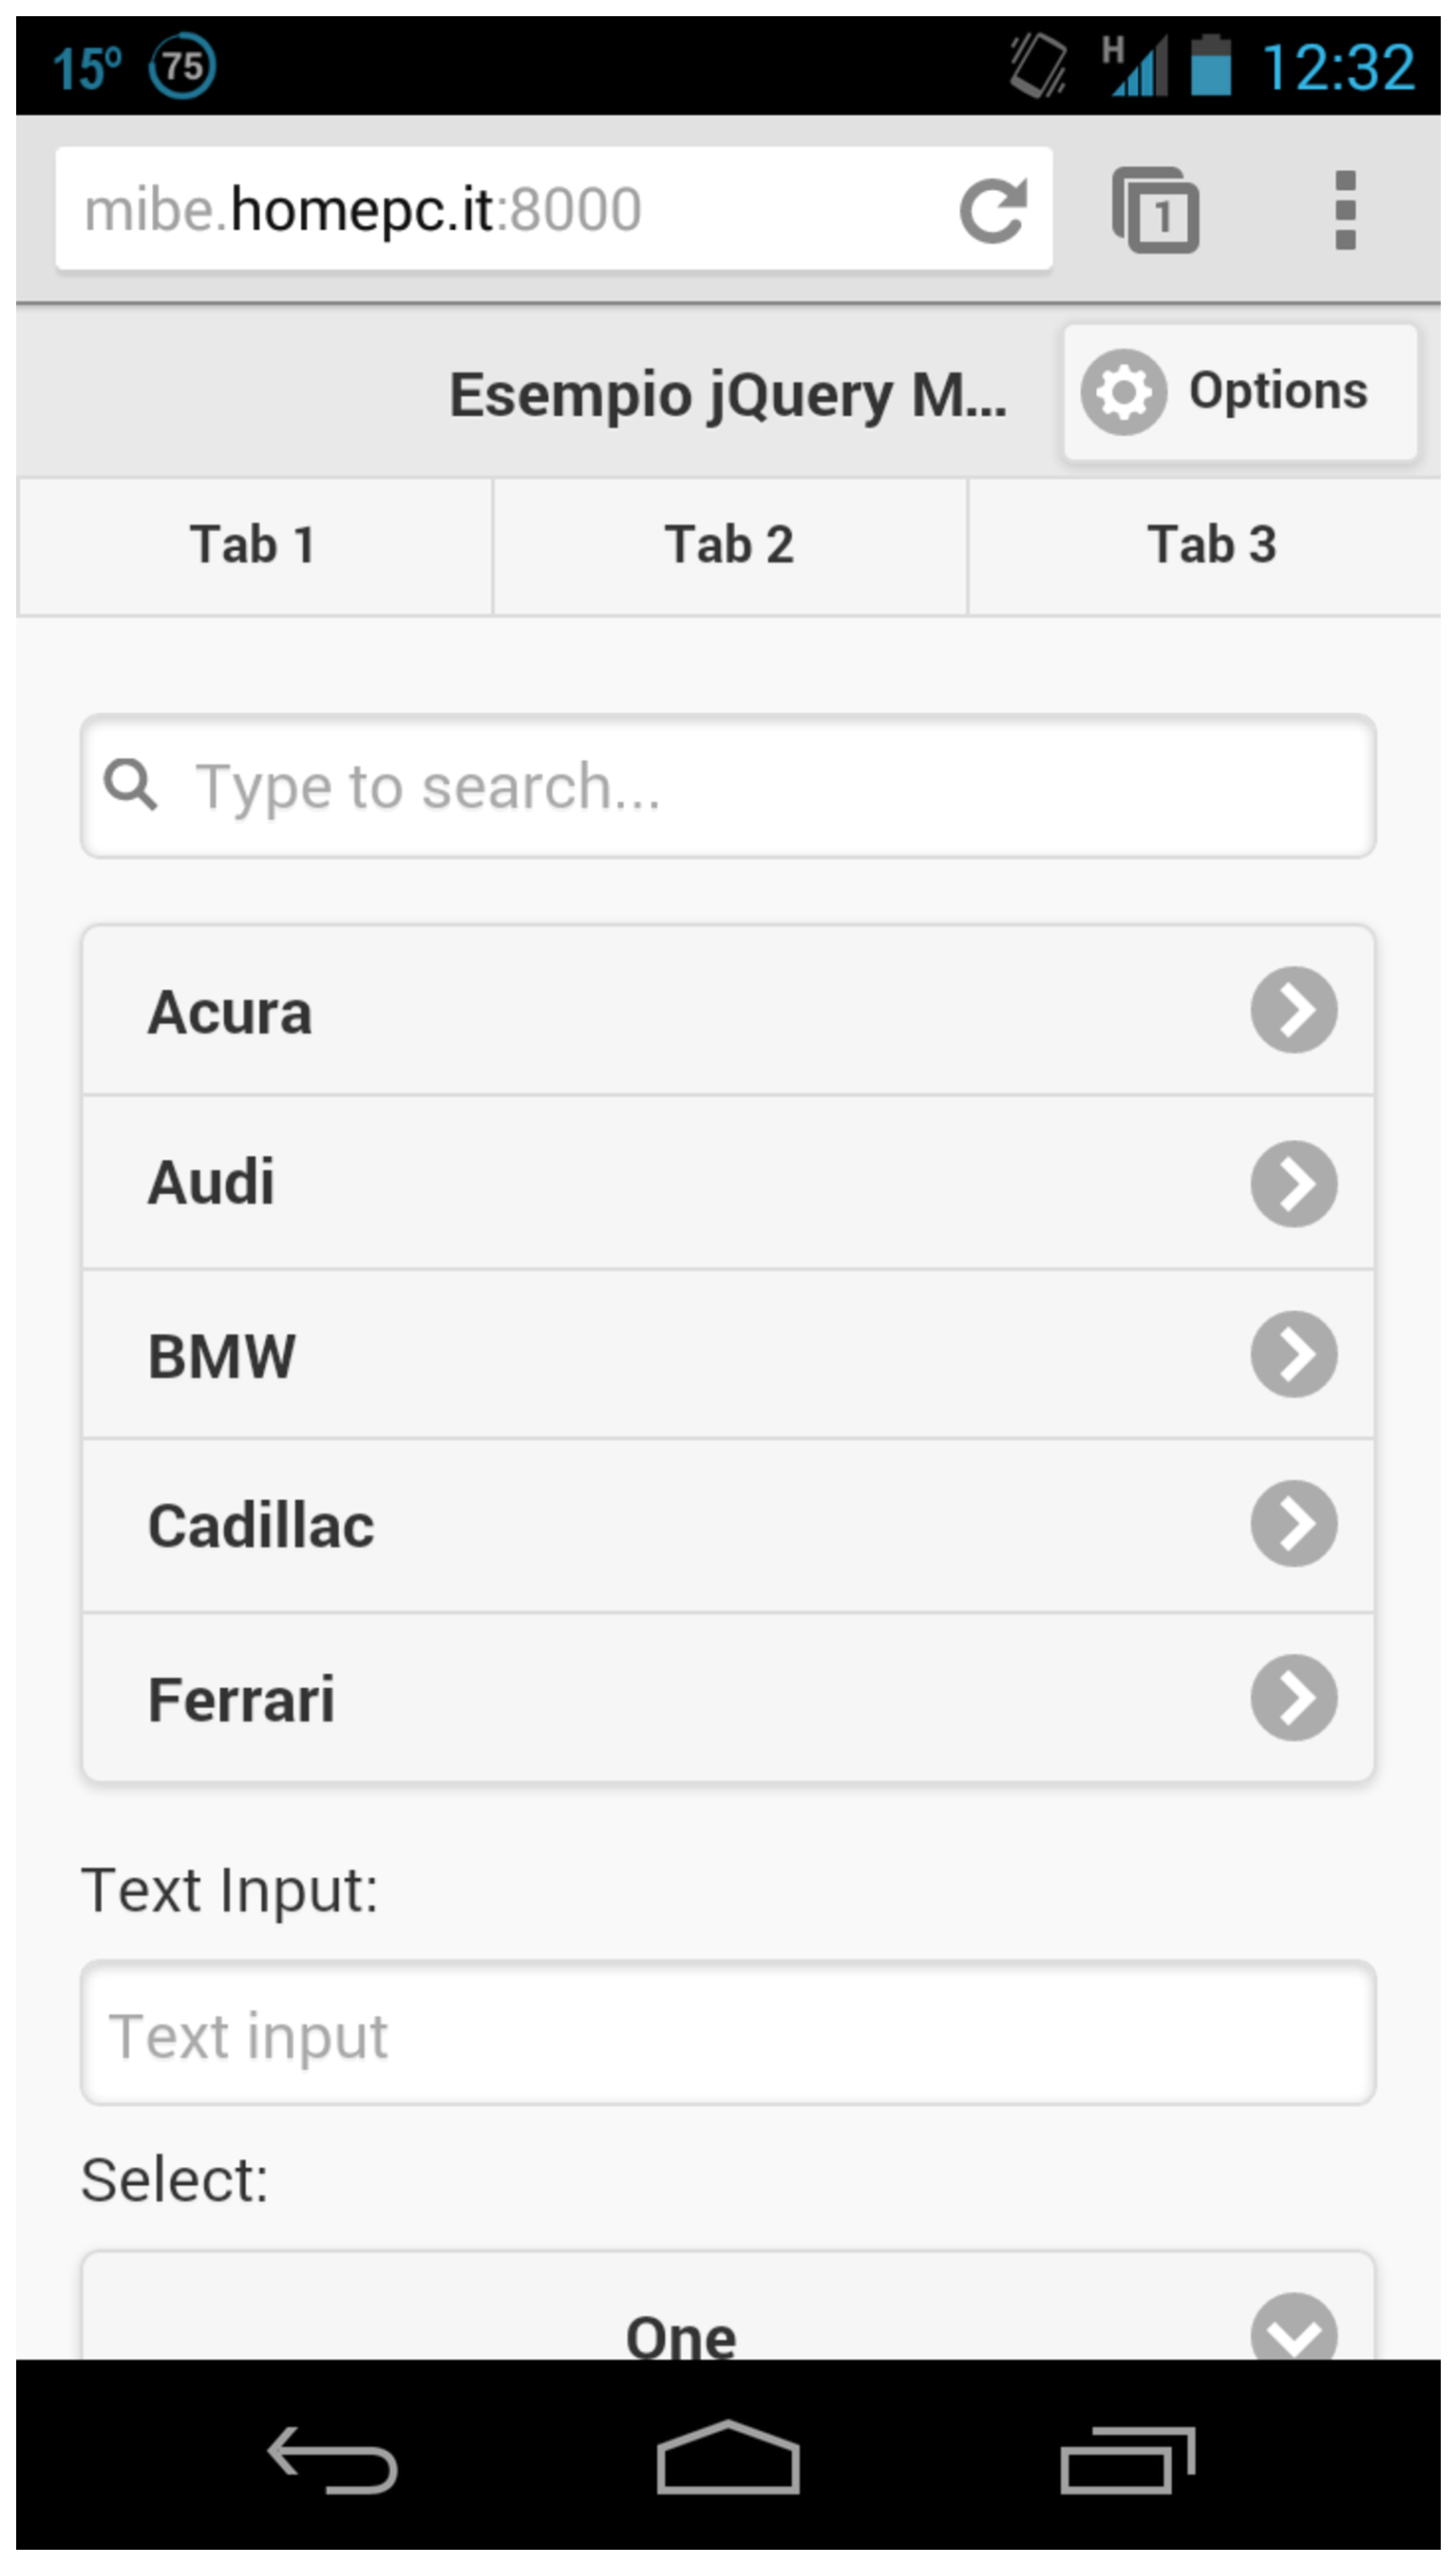
\includegraphics[keepaspectratio=true, width=0.32\textwidth]{jQuery-and}
				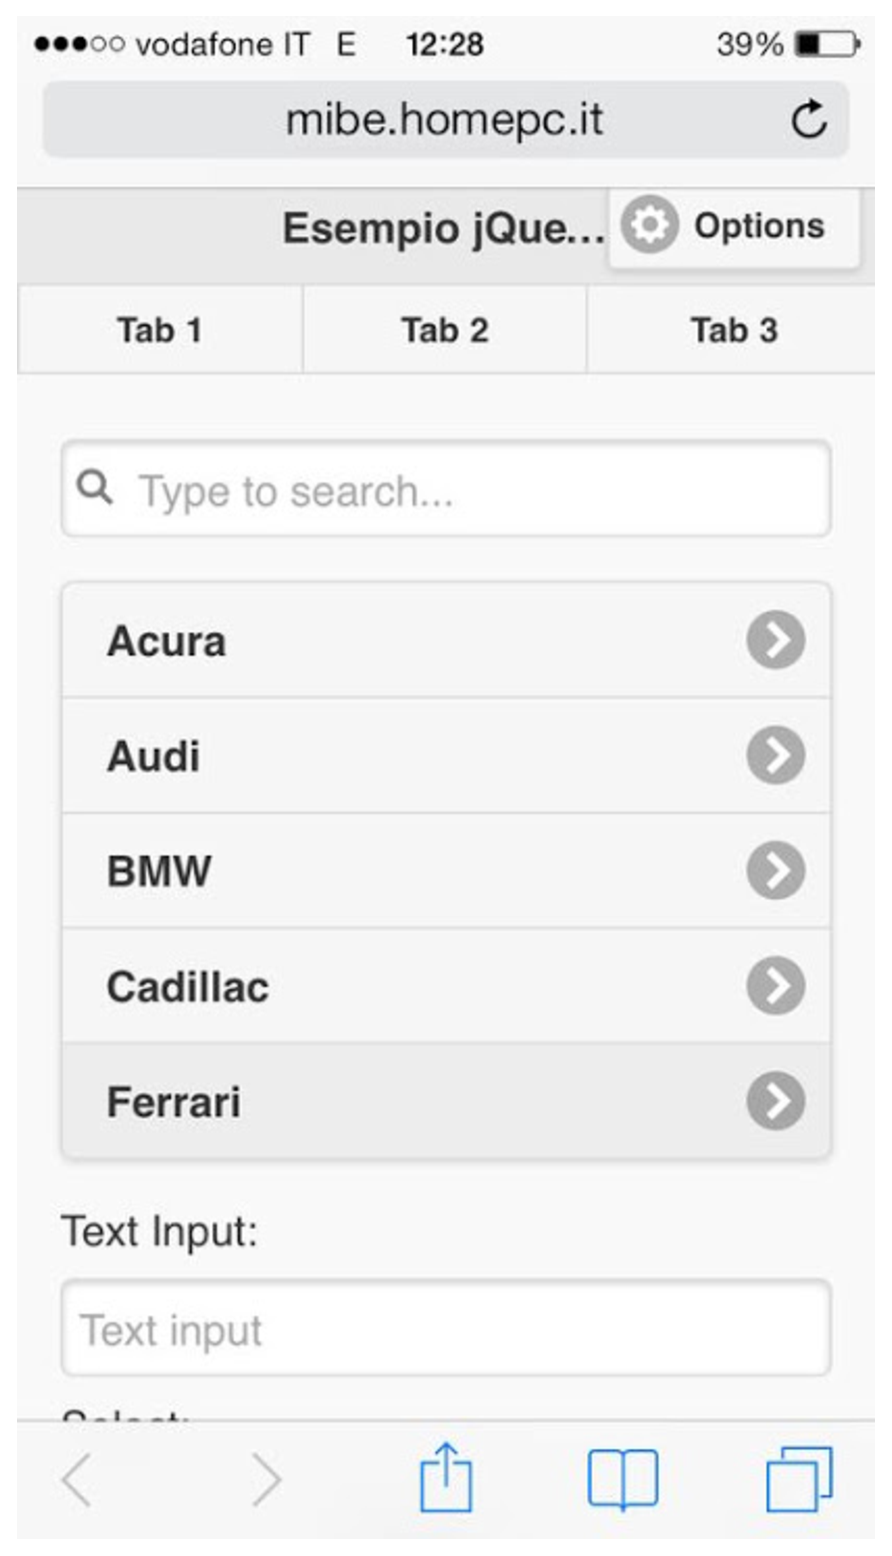
\includegraphics[keepaspectratio=true, width=0.32\textwidth]{jQuery-ios}
				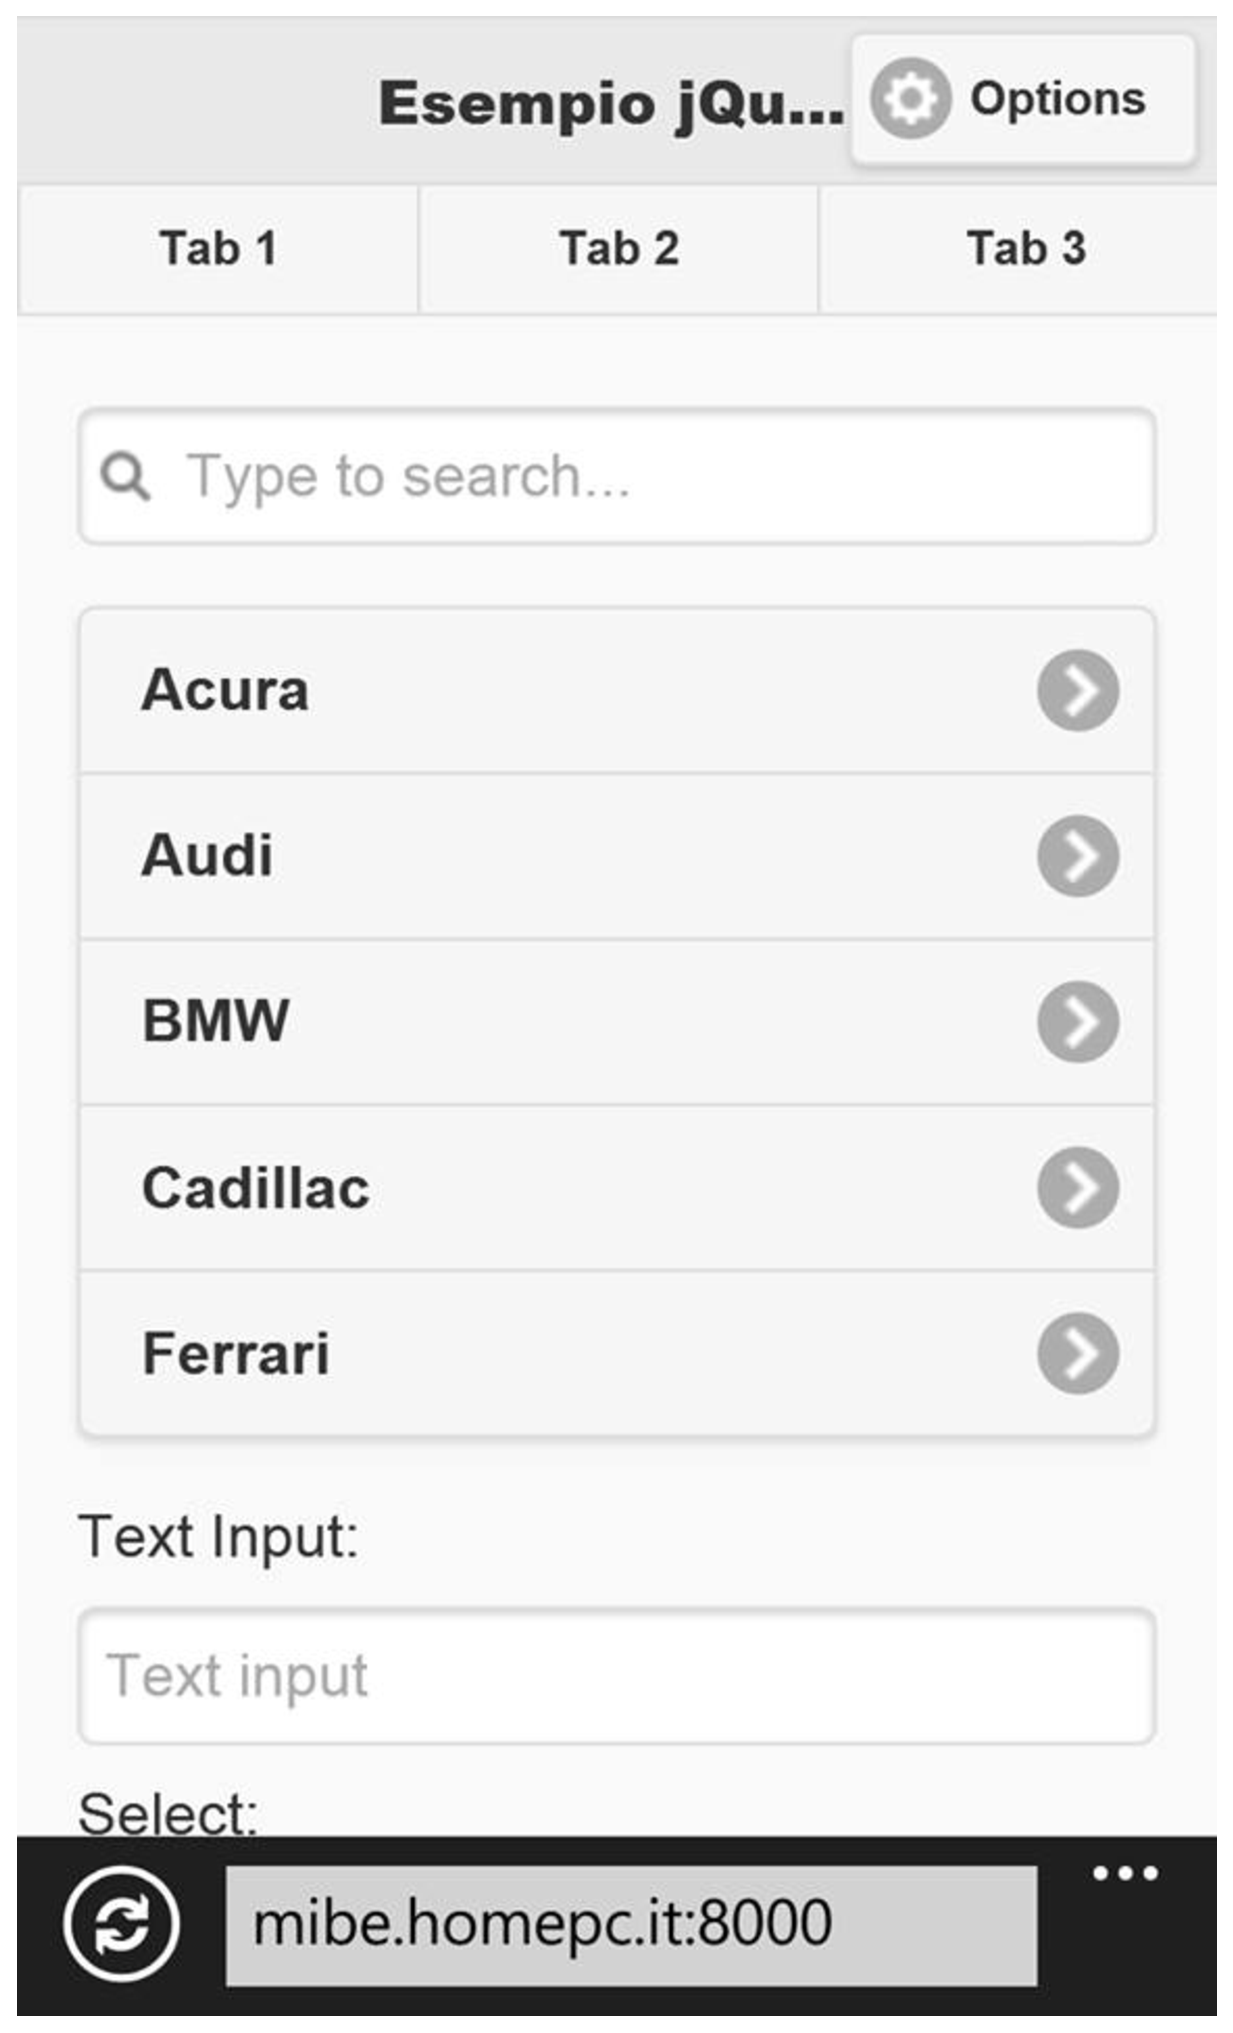
\includegraphics[keepaspectratio=true, width=0.32\textwidth]{jQuery-wp8}
				\caption{
					Un esempio di applicazione web realizzata con jQuery Mobile.
					Da sinistra a destra l'anteprima su piattaforma Android, iOS
					e WindowsPhone8.
				}
				\label{fig:jquery}
			\end{figure}
	
		\subsection{Kendo UI Mobile}
		\label{subsec:kendo}
			Kendo UI Mobile è un framework mobile completo che adatta
			automaticamente	l'aspetto dell'applicazione alla piattaforma sulla
			quale è eseguita. Consiste di estensioni fondamentali per un
			framework mobile come layouts, views, animazioni di transizione,
			ecc. oltre ad un insieme di widgets per	l'interfaccia grafica che
			includono bottoni, widgets per la navigazione, e altro. Non è però
			solo per queste caratteristiche che viene definito un framework
			completo, infatti Kendo UI Mobile offre anche: un solido componente
			DataSource, strumenti di validazione, API per la globalizzazione e
			un framework MVVM (Model View ViewModel). Come jQuery Mobile, Kendo
			è basato sulla libreria jQuery.
			
			Kendo UI Mobile in versione di prova è scaricabile dal sito 
			\url{http://www.telerik.com/download/kendo-ui-mobile}, quello che si 
			ottiene è un pacchetto zip contenente tutti i file JavaScript e CSS 
			necessari. La versione di prova	può essere usata per apprendere
			l'uso del frameworck ma non può essere usata per scopi commerciali 
			quindi, a differenza di jQuery Mobile, è necessario	mettere in conto
			la spesa di acquisto della licenza se si intende commercializzare
			l'applicazione.	I file JavaScript e CSS scaricati devono essere
			inseriti nel file HTML che costituisce l'applicazione esattamente
			come è stato descritto per jQuery Mobile\footnote{Informazioni
			aggiuntive per iniziare a lavorare con kendo UI Mobile si possono
			trovare nel sito \url{http://docs.telerik.com/kendo-ui/getting-started/introduction}}.
			
			Il punto di forza di Kendo UI Mobile è la possibilità di creare
			applicazioni con aspetto nativo. Scrivendo codice una sola volta
			sarà infatti il framework, all'avvio dell'applicazione, ad occuparsi
			di identificare la piattaforma e a applicare il tema corretto. A
			prescindere da questa funzionalità è comunque possibile forzare
			l'utilizzo di uno stesso tema su piattaforme diverse. Attualmente
			Kendo UI Mobile fornisce temi di aspetto nativo per le piattaforme
			Android, iOS, BlackBerry e Windows Phone 8 come mostrato in figura~
			\ref{fig:kendoui} ma, se si ha la necessità, è disponibile uno
			strumento online per la realizzazione dei propri temi
			personalizzati.
			\begin{figure}
				\centering
				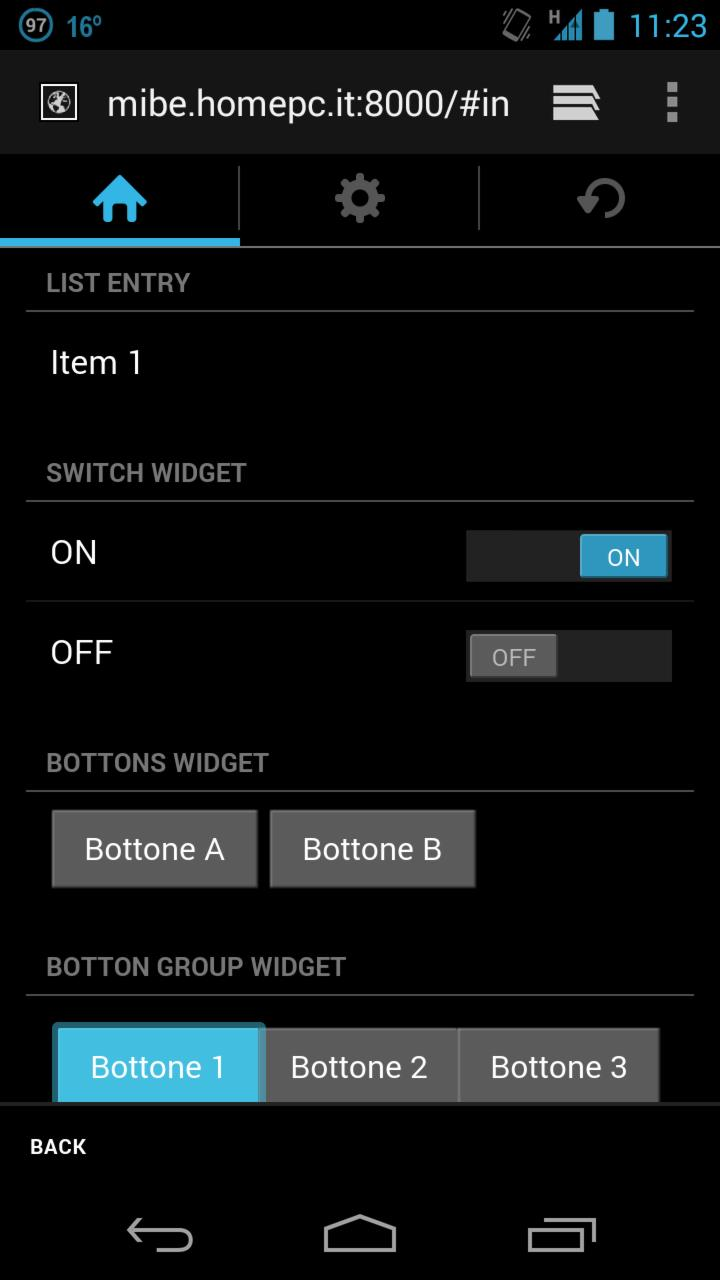
\includegraphics[keepaspectratio=true, width=0.32\textwidth]{kendoui-and}
				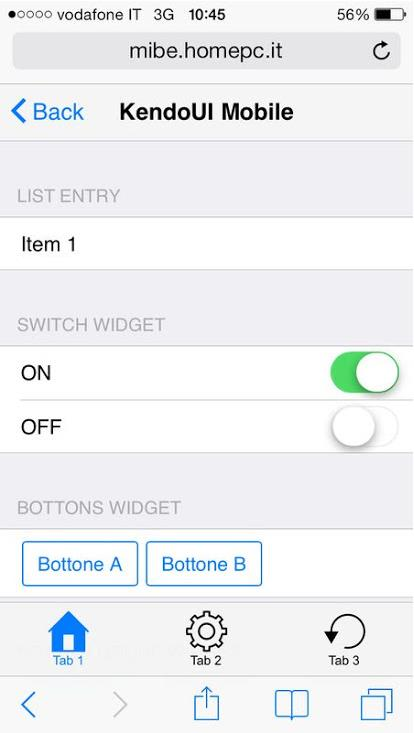
\includegraphics[keepaspectratio=true, width=0.32\textwidth]{kendoui-ios}
				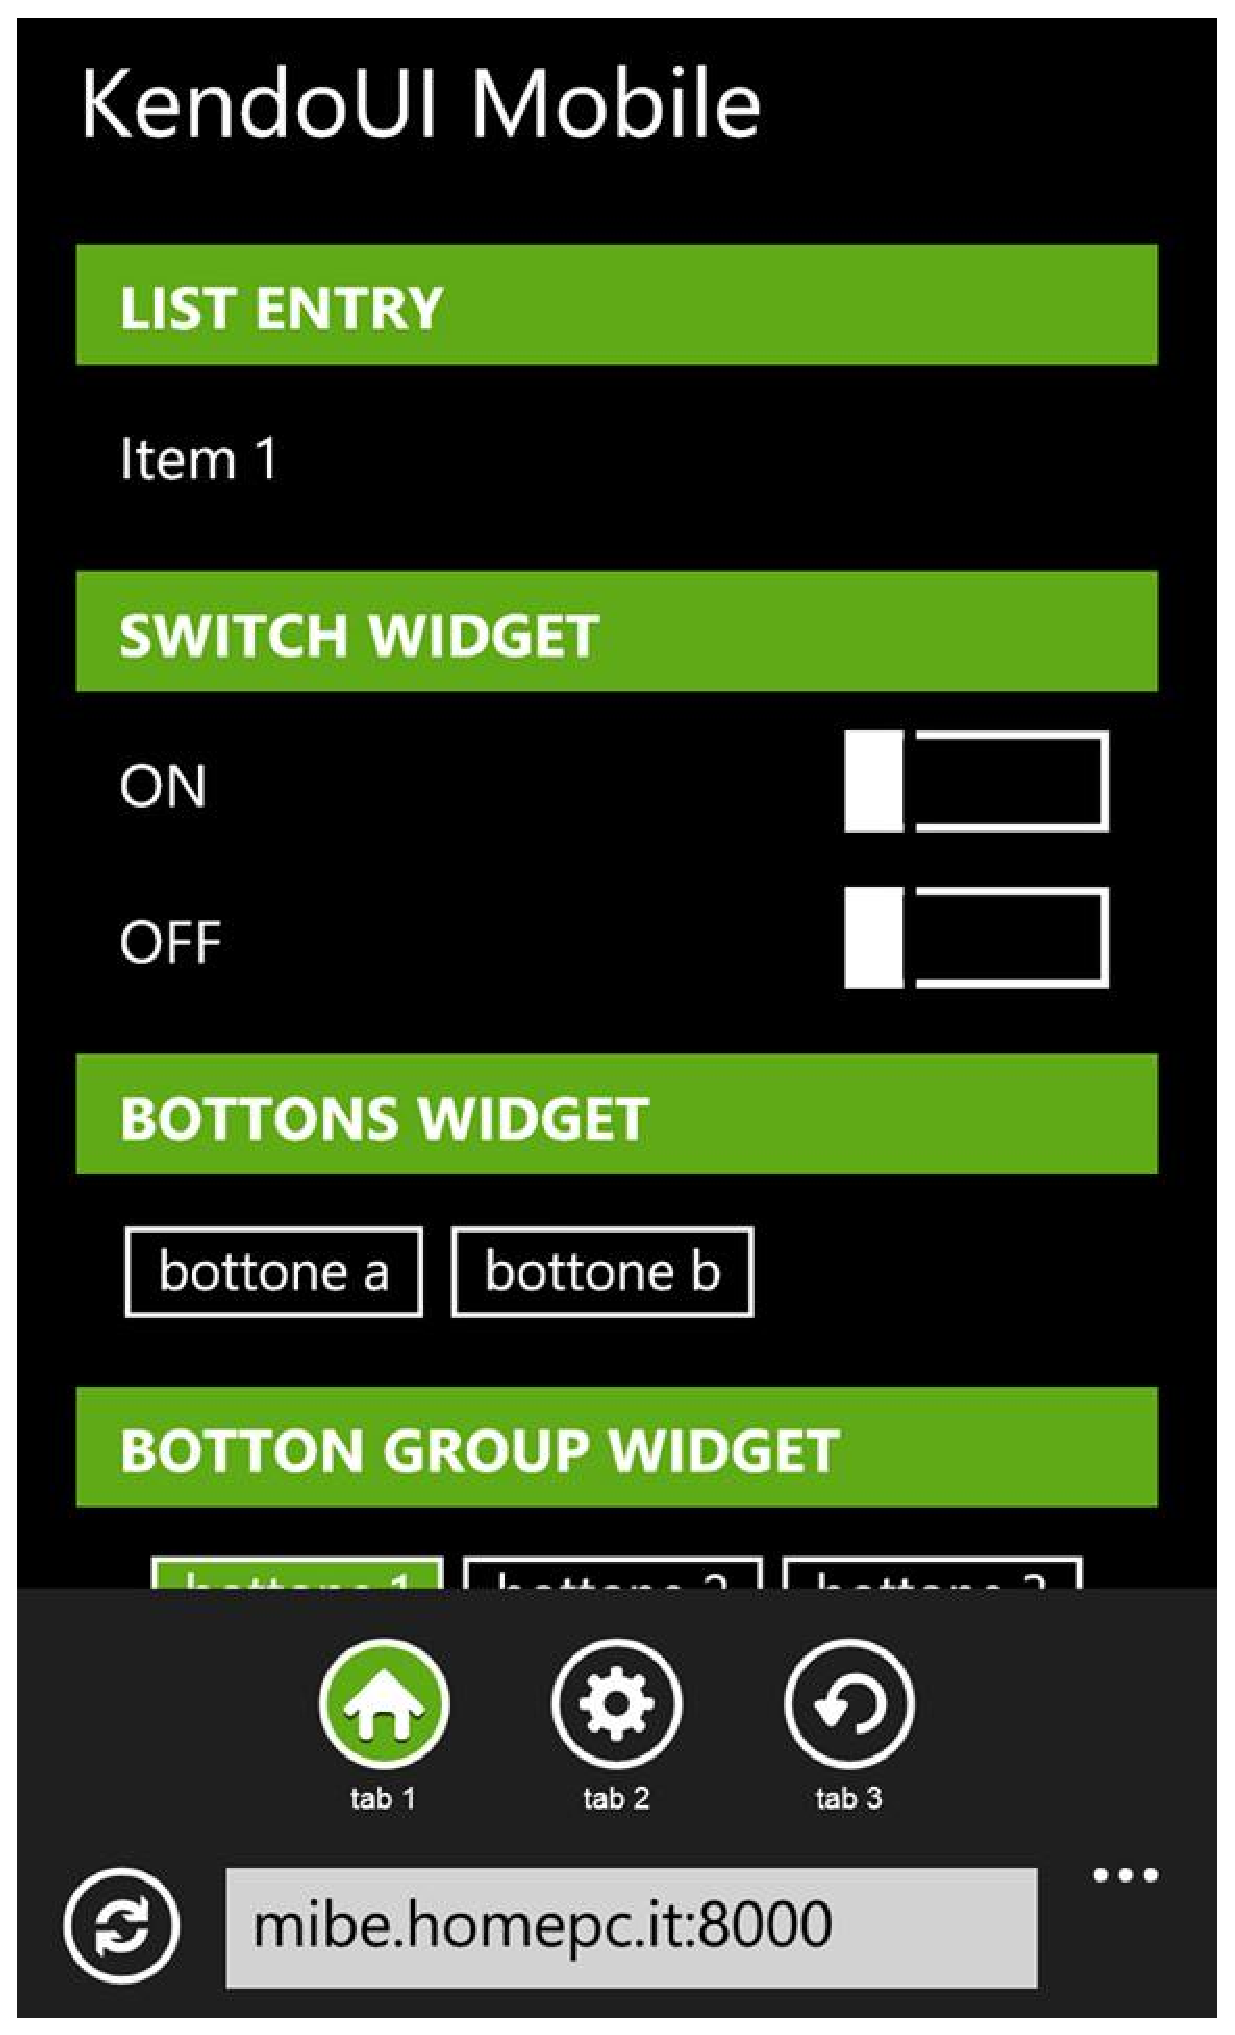
\includegraphics[keepaspectratio=true, width=0.32\textwidth]{kendoui-wp8}
				\caption{
					Un esempio di applicazione web realizzata con KendoUI Mobile.
					Da sinistra a destra l'anteprima su piattaforma Android, iOS
					e WindowsPhone8.
				}
				\label{fig:kendoui}
			\end{figure}
			ThemeBuilder\footnote{Disponibile online sul sito web del produttore
			all'indirizzo \url{http://demos.telerik.com/kendo-ui/themebuilder/mobile.html}}
			con una semplice interfaccia grafica permette di modificare colori e
			sfondi alle componenti grafiche dell'applicazione mostrando
			un'anteprima per ogni piattaforma supportata; una volta ottenuto il
			risultato desiderato è possibile esportare il tema in un file CSS da
			utilizzare poi nella nostra app.
			
			Come precedentemente detto Kendo UI Mobile non offre solo elementi
			di personalizzazione per l'interfaccia grafica. Il componente
			DataSource (Kendo UI DataSource) è un'astrazione per usare dati
			locali (array di oggetti JavaScript) o remoti (XML, JSON, JSONP).
			Esso supporta completamente il CRUD (Create, Read, Update, Destroy)
			cioè fornisce la funzioni per creare, leggere, aggiornare e
			distruggere dati e permette, sia alla parte locale che alla parte
			server, di ordinare	impaginare, filtrare, raggruppare e aggregare
			questi dati. Molti widgets di Kendo UI supportano il data binding,
			cioè l'associazione dei dati agli elementi grafici; grazie a questo
			è possibile ad esempio mostrare in una lista i dati letti da un
			server o caricati localmente.

			Come detto poco fa KendoUI Mobile fornisce un framework per lo
			sviluppo seguendo il paradigma MVVM; per provare a spiegare in cosa
			consiste tale modello ci serviamo di un esempio: in un qualsiasi
			genere di programma o applicazione tipicamente è cosa comune dover
			manipolare certe entità; un'app che gestisce domande di laurea dovrà
			ragionevolmente trattare studenti, dove uno studente avrà 
			particolari caratteristiche come nome, cognome e numero di matricola.
			Questo avrà due rappresentazioni: una in memoria mediante strutture
			dati opportune e un'altra grafica dove i dati dello studente saranno
			mostrati all'utente attraverso elementi grafici. L'utente può
			inoltre compiere determinate azioni su queste entità attraverso
			elementi grafici (es. sottoporre la domanda di laurea attraverso
			il tocco di un apposito tasto). Il paradigma Mo\-del-\-View-\-View\-Mo\-del 
			formalizza le suddette rappresentazioni rispettivamente come Model e 
			View, inoltre introduce il ViewModel, un terzo elemento che le mette 
			in relazione, consentendo che le azioni e le modifiche fatte da
			parte dell'utente sulla View si ripercuotano sul relativo Model e
			viceversa. Strutturare un applicazione separandola in queste parti
			si ottiene un codice più strutturato, più manutenibile nonché più
			leggibile.
			
			Kendo fornisce un modo per internazionalizzare le pagine che 
			compongono l'applicazione. Attraverso un particolare metodo offerto
			dalle API di Kendo è possibile selezionare un particolare paese in 
			modo da adottare formato dei numeri, nomi dei mesi, formato 
			di data e ora e altro conformemente agli standard locali.
	
			HTML5 ha introdotto gli attributi di validazione, questi particolari 
			attributi hanno la capacità di forzare il browser ad avvisare
			l'utente che un certo elemento di input contenuto in un form debba
			essere compilato obbligatoriamente.	Kendo UI Validator offre un modo
			facile per gestire la validazione per gli elementi input di un form
			permettendo di personalizzare la gestione della validazione, ad
			esempio, accettando in input solo stringhe contenenti certe parole o
			numeri compresi in un dato intervallo.
			
			Come in jQuery Mobile è possibile realizzare l'intera applicazione 
			in una singola pagina HTML che, attraverso il widgets view, si è in 
			grado di suddividere in più schermate. Ad ogni view può essere data
			una particolare struttura, in particolare è possibile suddividerla
			in un'intestazione e un corpo. La stessa struttura può essere
			condivisa tra più views	permettendo di usare l'intestazione per
			navigare tra le schermate in quei dispositivi (es. iPhone) dove non
			esistono tasti fisici appositi. Tutto questo contribuisce ad
			avvicinare l'esperienza utente a quella di una reale applicazione
			nativa. I vantaggi di scrivere l'applicazione all'interno di una
			sola pagina	HTML sono gli stessi discussi per jQuery Mobile 
			\hyperref[subsec:jQuery]{(vedi~\ref{subsec:jQuery})}.
			
		\subsection{PhoneJS}
			PhoneJS è un framework per realizzare applicazioni mobili 
			single page application (SPA), che promette di fornire: un'
			esperienza utente ottimizzata per i dispositivi touch, widgets con 
			aspetto nativo, agili strumenti di navigazione tra le schermate dell'
			applicazione, facile gestione delle schermate e un livello di accesso 
			ai dati.
			
			La libreria PhoneJS sfrutta completamente jQuery e opzionalmente 
			supporta KnockoutJS, per sviluppare l'applicazione attraverso il paradigma 
			MVVM\hyperref[subsec:kendo]{(vedi~\ref{subsec:kendo})}.
			L'obiettivo è sempre quello di realizzare un'applicazione web cross-platform 
			riusando completamente il codice.
			
			Come Kendo UI, questo framework è in grado di fornire all'applicazione 
			un aspetto differente a seconda del dispositivo senza scrivere codice aggiuntivo.
			PhoneJS, infatti, identifica la piattaforma a tempo di esecuzione 
			e applica automaticamente 
			lo stile "nativo" appropriato a tutti i widgets e a tutti gli elementi 
			di navigazione (riferimento a immagine)
			
			PhoneJS include un vasto insieme di widgets (elementi UI). Tipicamente, 
			un widget è associato a dei dati e fornisce un'interazione con l'utente.
			Esso è rappresentato da un elemento HTML (contenitore), da un codice 
			JavaScript per definirne il comportamento e dei fogli di stile CSS. 
			Ogni widget include un plugin jQuery e un legame Knockout, è così 
			possibile scegliere se creare un widget attraverso l'approccio jQuery 
			oppure usare le funzionalità di tracciamento delle dipendeze (?) fornito 
			da KnockoutJS. 
			
			PhoneJS fornisce tutti gli strumenti necessari per realizzare un'applicazione 
			SPA: gestione e rendering delle schermate, navigazione attraverso url, 
			layout specifico per il dispositivo, caching delle view e gestione degli stati.
			Il framework usa le familiari regole di navigazione per definire la 
			relazione tra l'URL nel quale l'utente naviga e la corrispondente schermata 
			da caricare. Lo sviluppatore deve specificare la regola di navigazione e definire 
			la schermata dell'applicazione, il framework a run-time si occuperà di effettuare la 
			navigazione.
			Quando si naviga in una view, questa sarà resa visibile attraverso un 
			animazione di transizione, inoltre il framework tiene traccia dell'avvenuta 
			navigazione e aggiunge un bottone per tornare indietro. Questo comportamento 
			di default può comunque essere cancellato.
			
			Per migliorare l'esperienza di sviluppo con PhoneJS è possibile usare 
			il pacchetto DXTREME. Esso include le librerie PhoneJS e ChartJS e il 
			supporto per Visual Studio 2012. Inoltre include un emulatore basato 
			su browser che permette di fare debugging direttamente da Visual Studio.
			DXTREME non è gratis, ma è possibile usarne una versione di prova per 
			30 giorni.
			
	\section{Framework per Applicazioni Ibride}
	\label{sec:frameworkhybrid}
		\subsection{Phonegap}
			Lo scopo di PhoneGap è di permettere alle applicazioni web di essere 
			installate sui dispositivi come avviene per le applicazioni native. 
			Phonegap crea un'applicazione nativa consistente principalmente in 
			una web view, e al suo interno ci racchiude l'applicazione web. Il pacchetto 
			risultante è un file che può essere installato attraverso gli app stores
			proprio come le applicazioni native.
			Addizionalmente, PhoneGap fornisce un insieme di API che comunemente non 
			sono disponibili alle applicazioni web, come: accesso alla fotocamera, 
			ai contatti e ai sensori.
			
			Per sviluppare le applicazioni con PhoneGap, gli sviluppatori devono 
			creare un'applicazione web, questo può essere fatto usando i framework 
			descritti sopra.  
			
			Per eseguire un'applicazione su un emulatore (simulatore per iOS), 
			lo sviluppatore deve generare il pacchetto per ogni piattaforma che 
			vuole supportare utilizzando gli SDK opportuni.
			
			Per alleviare la necessità di dover installare localmente 
			tutti gli SDKs nativi 
			per le piattaforme per cui si intende sviluppare, Nitobi (recentemente 
			aquistata da Adobe) ha creato un servizio chiamato PhoneGap Build. 
			Inviando i sorgenti HTML, CSS e JavaScript al servizio, attraverso un 
			pacchetto .zip o attraverso il repository GitHub, è possibile ottenere 
			l'applicazione installabile sulle varie piattaforme.
			L'attuale versione di PhoneGap Build è la 3.1.0 ed è in grado di compilare 
			applicazioni per iOS, Android e WindowsPhone 8. Per iOS serve comunque 
			essere registrati tra gli sviluppatori Apple questo consentirà di 
			testare le app su iPhone e iPad. Per essere uno sviluppatore 
			registrato Apple, occorre pagare una tassa di iscrizione annuale 
			pari a 79 euro.
			Oltre alla possibilità di fare compilazione PhoneGap Build fornisce 
			il cosiddetto Hydration, un'opzione di compilazione che se abilitata 
			permette di testare le modifiche fatte all'applicazione senza doverla 
			reinstallare sul dispositivo (attenzione non tutte le modifiche 
			funzionano). Infine PhoneGap Build offre un server weinre per fare 
			debugging in remoto, usando gli strumenti di debug tipici dello 
			sviluppo web.
			 
			Il processo di sviluppo con PhoneGap Build da una parte permette di 
			poter iniziare a realizzare l'applicazione senza perder tempo a 
			installare e configurare tutti gli SDK nativi, ma allo stesso tempo 
			abbiamo notato che il servizio è molto lento, sia per il tempo speso  
			ad inviare il codice sorgente e a scaricare il pacchetto, sia perchè 
			il processo 
			di build non sembra essere molto performante e spesso il sito mostra 
			dei disservizi. Inoltre bisogna tener conto che non tutti i plugin 
			esistenti per PhoneGap/Cordova sono utilizzabili con il servizio 
			PhoneGap Build, anche se la possibilità di aggiungere plugin di terze 
			parti sta facendo crescere il numero di quelli disponibili.
			
			Come menzionato precedentemente, un'applicazione PhoneGap è un 
			"contenitore nativo" di un'applicazione web. Proviamo a spiegarci 
			meglio.
			Molti SDKs nativi forniscono un particolare elemento grafico chiamato 
			"Web View", all'interno del quale è possibile caricare del contenuto 
			HTML, CSS e JavaScript che viene interpretato come se fosse stato aperto in 
			un Browser. 
			PhoneGap fondamentalmente carica le pagine HTML dell'applicazione web 
			in uno di questi Web View. L'applicazione nativa che crea il web view 
			è in grado di (in maniera differente a seconda della piattaforma) 
			comunicare in maniera asincrona col codice JavaScript eseguito nel 
			web view. 
			PhoneGap sfrutta questa funzionalità per creare API JavaScript 
			che sono in grado di scambiare mesaggi asincroni col codice 
			nativo da dentro la web view.  
			Il modo in cui tutto questo è implementato è diverso a seconda della 
			piattaforma, e non è scopo di questa relazione scenderne troppo nei 
			dettagli, dettagli più significativi possono essere trovati su 
			(mettere un link a dove sono spiegati).
			
			La principale forza di PhoneGap risiede nella sua semplicità. 
			Il team di sviluppatori di PhoneGap ha intenzionalmente implementato 
			solo il minimo comune denominatore delle APIs native. In questo modo 
			è facile per PhoneGap supportare molte piattaforme. Potenzialmente 
			una qualsiasi piattaforma che offre una web view può essere supportata 
			da PhoneGap.
			Inoltre le API di PhoneGap possono essere estese con dei plug-in, cioè 
			è possibile implementare personalmente l'accesso a particolare API native.
			(citazione di qualche plugin)
			
			La qualità dell'intefaccia untente in un'applicazione PhoneGap 
			varia in base al framework usato per realizzare la web app, e al 
			motore di rendering delle pagine web della piattaforma.
			Il motore di rendering WebKit su iOS fornisce buone performance, le 
			Android Web View sono funzionali, ma ha qualche notabile limitazione 
			(citare fonte).
			

		\subsection{Rho Mobile}
			Descrizione Rho Mobile

		\subsection{Sencha Touch}
			Descrizione Sencha Touch
	
	\section{Conclusioni}
		Per questo motivo e quello... abbiamo scelto di realizzare una app di 
		prova con Phonegap e Titanium.
